\documentclass[10pt, a5paper]{article}
\usepackage[T2A]{fontenc}
\usepackage{ucs}
\usepackage[utf8x]{inputenc}
\usepackage[polish,english,russian]{babel}
\usepackage{hyperref}
\usepackage[inner=2cm,top=1.8cm,outer=2cm,bottom=2.3cm,nohead]{geometry}
\usepackage{listings}
\usepackage{graphicx}
\usepackage{wrapfig}
\usepackage{longtable}
\usepackage{indentfirst}
\frenchspacing
\usepackage{fixltx2e} %text sub- and superscripts
\usepackage{icomma} % коскі ў матэматычным рэжыме
\PreloadUnicodePage{4}

\newcommand{\longpage}{\enlargethispage{\baselineskip}}
\newcommand{\shortpage}{\enlargethispage{-\baselineskip}}

\def\switchlang#1{\expandafter\csname switchlang#1\endcsname}
\def\switchlangbe{
\let\saverefname=\refname%
\def\refname{Літаратура}%
\def\figurename{Іл.}%
}
\def\switchlangen{
\let\saverefname=\refname%
\def\refname{References}%
\def\figurename{Fig.}%
}
\def\switchlangru{
\let\saverefname=\refname%
\let\savefigurename=\figurename%
\def\refname{Литература}%
\def\figurename{Рис.}%
}

\hyphenation{admi-ni-stra-tive}
\hyphenation{ex-pe-ri-ence}
\hyphenation{fle-xi-bi-li-ty}
\hyphenation{Py-thon}
\hyphenation{ma-the-ma-ti-cal}
\hyphenation{re-ported}
\hyphenation{imp-le-menta-tions}
\hyphenation{pro-vides}
\hyphenation{en-gi-neering}
\hyphenation{com-pa-ti-bi-li-ty}
\hyphenation{im-pos-sible}
\hyphenation{desk-top}
\hyphenation{elec-tro-nic}
\hyphenation{com-pa-ny}
\hyphenation{de-ve-lop-ment}
\hyphenation{de-ve-loping}
\hyphenation{de-ve-lop}
\hyphenation{da-ta-ba-se}
\hyphenation{plat-forms}
\hyphenation{or-ga-ni-za-tion}
\hyphenation{pro-gramming}
\hyphenation{in-stru-ments}
\hyphenation{Li-nux}
\hyphenation{en-vi-ron-ment}
\hyphenation{Te-le-pathy}
\hyphenation{Li-nux-ov-ka}

\def\progref!#1!{\texttt{#1}}
\renewcommand{\arraystretch}{2} %Іначай формулы ў матрыцы зліпаюцца з лініямі
\usepackage{array}

\def\interview #1 (#2), #3, #4, #5\par{

\section[#1, #3, #4]{#1, #5}
\def\qname{LVEE}
\def\aname{#1}
\def\q ##1\par{{\noindent \bf \qname: ##1 }\par}
\def\a{{\noindent \bf \aname: } \def\qname{L}\def\aname{#2}}
}

\begin{document}
\title{Любительская малобюджетная аэрофотосъёмка с использованием свободного программного обеспечения}
\author{Дмитрий Самсонов, Москва, РФ\footnote{\url{samson.samson.samson@gmail.com}, \url{http://lvee.org/ru/abstracts/161}}}
\maketitle
\begin{abstract}
This work concerns some tasks needed for KAP (Kite Aerial Photography) with free/libre software (mostly from Debian \linebreak GNU/Linux). This method was successfully used for taking aerial photos of several open-airs in 2013 and 2014. Nowadays it is very important to have cheap and simple solution. 
\end{abstract}
Иногда возникает необходимость сделать аэрофотосъёмку. Например, на фестивале, проводящемся на открытом воздухе. Свежепостроенные фестивальные объекты могут не попасть на общедоступные спутниковые снимки, поэтому снимать их приходится самостоятельно. В данной работе рассмотрена методика, применявшаяся при аэрофотосъёмке фестивалей <<Пустые Холмы "--- Город Золотой>> осенью 2013 года и <<Фестиваля 17>> летом 2014 года.

Задача состоит в том, чтобы, подняв фотоаппарат на достаточную высоту, сделать серию вертикальных снимков, после чего <<склеить>> их между собой, привязать к местности и привести в удобную для дальнейшей работы форму.

Немаловажна в наше время низкая стоимость как создания, так и эксплуатации решения подобной задачи.

\begin{figure}[h!]
  \centering \label{samsonov1}
  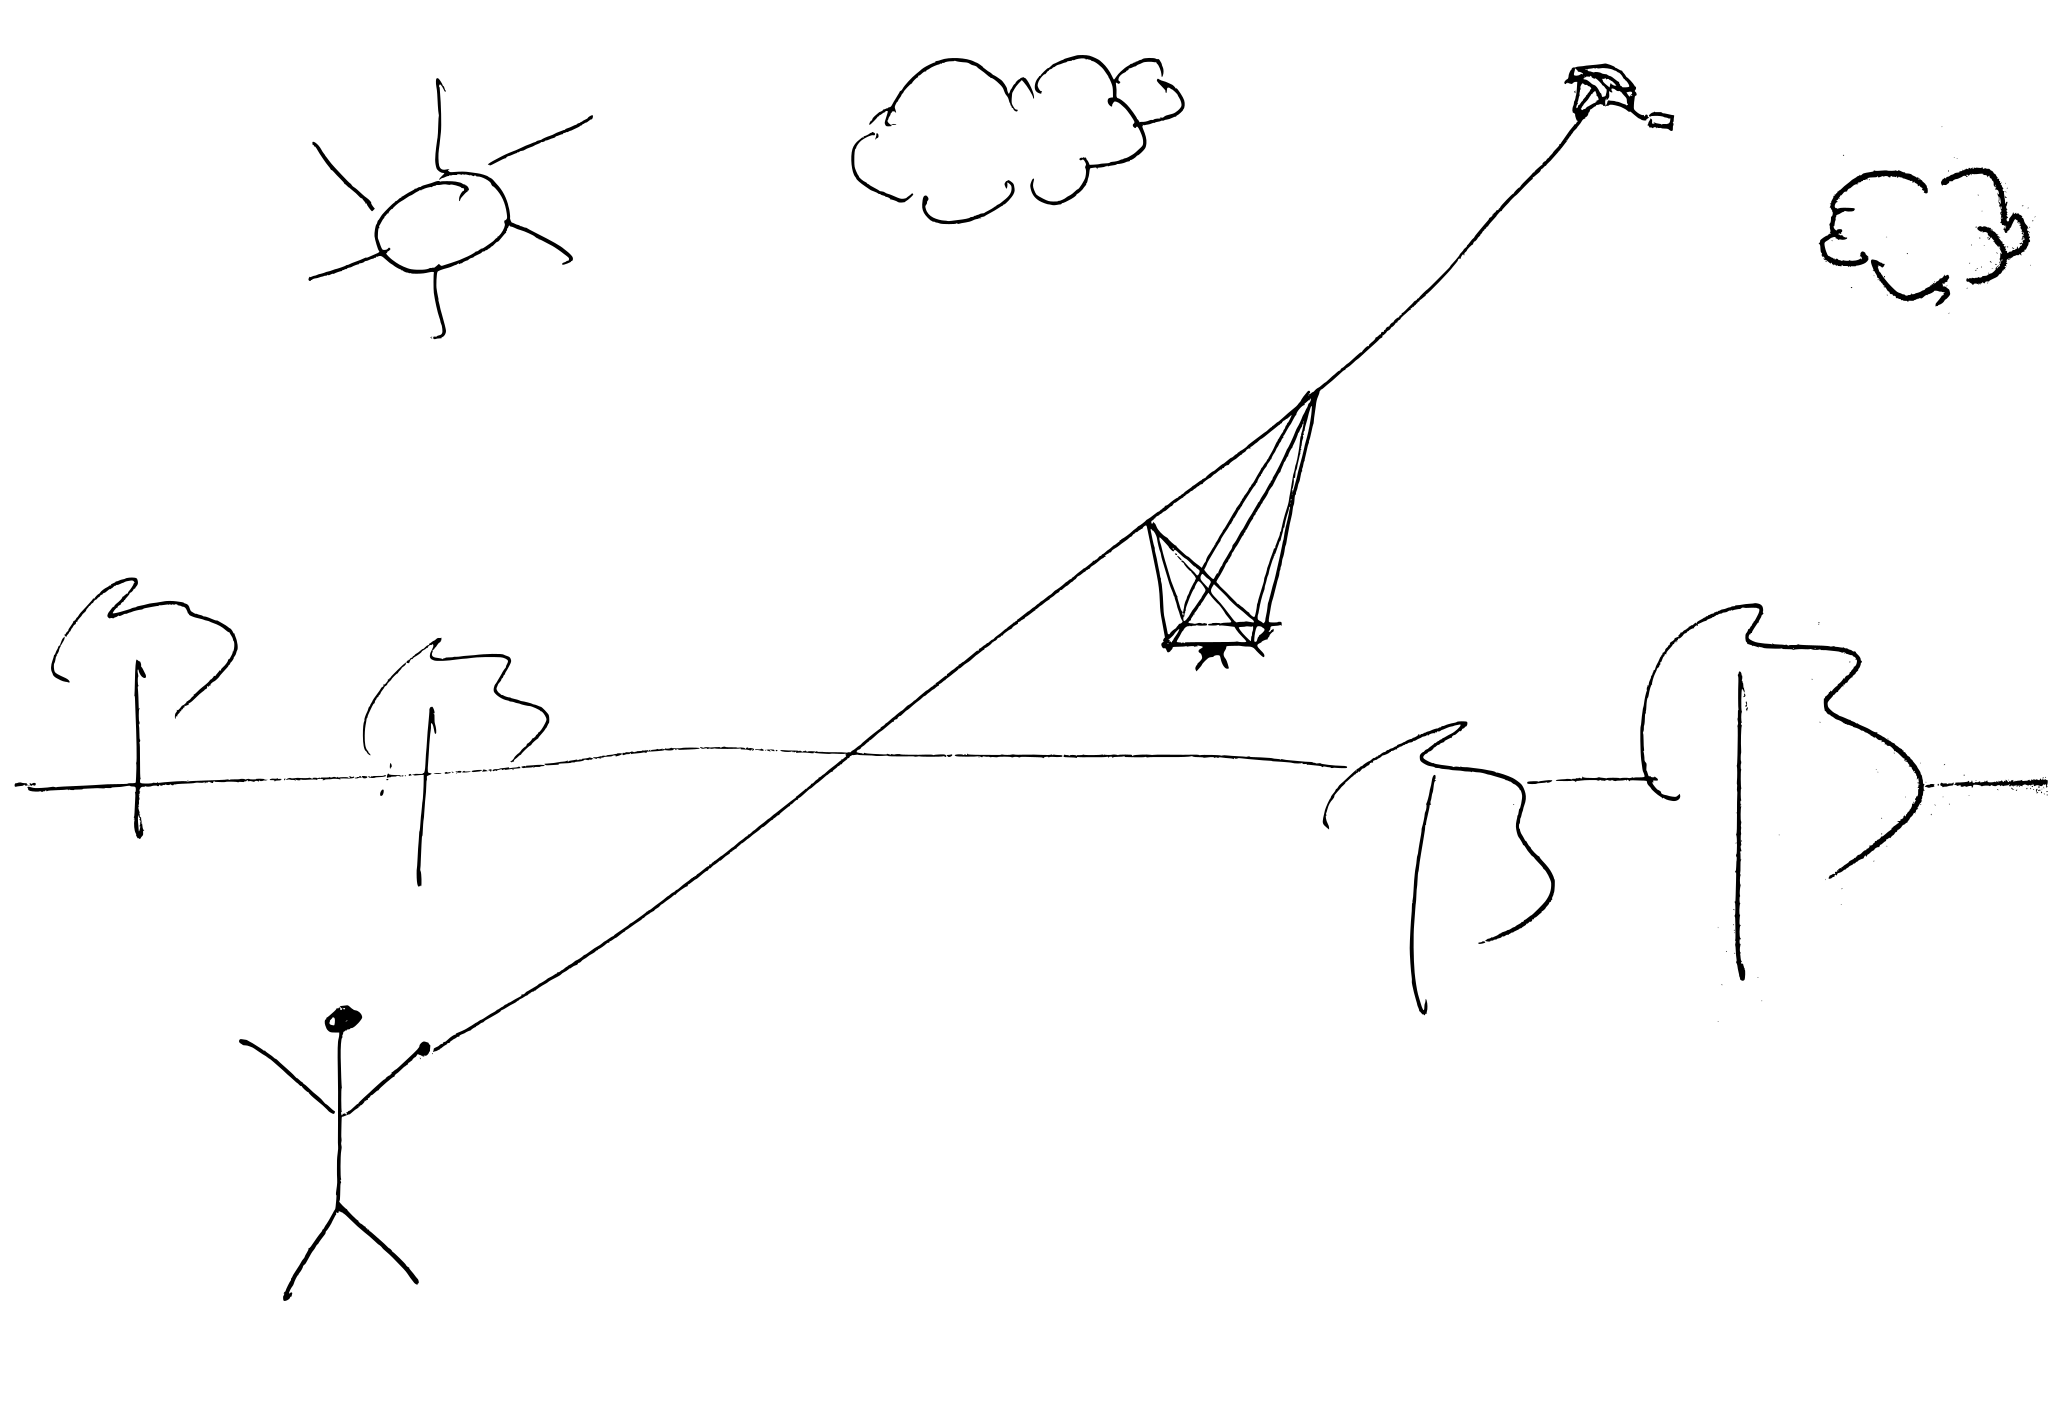
\includegraphics[scale=0.1]{14_2015_fig1}
  \caption{Схематичное изображение процесса аэрофотосъёмки}
\end{figure}


\section*{Аппаратная часть}

Готовые решения в виде специализированных самолётов стоят довольно дорого, а в самостоятельном производстве трудозатратны. Радиоуправляемые вертолёты (<<дроны>>) стоят дешевле, однако дрон, способный устойчиво поднимать в воздух относительно тяжёлый фотоаппарат, стоит существенно дороже дешёвых моделей (а лёгкие фото-видеокамеры дороги сами по себе). К тому же у дронов высокие эксплуатационные издержки. Относительно дешёвы конструкции типа \emph{воздушный змей} и \emph{воздушный шар}. Был выбран первый тип.

Для создания \emph{пикавета} "--- платформы, обеспечивающей вертикальность съёмки "--- была использована часть деревянной коробки, найденная среди бытовых отходов. Крючки для прикрепления пикавета к лееру были найдены в заброшенном цеху НИИДАРа (научно"=исследовательский институт дальней радиосвязи).

\begin{figure}[h!]
  \centering \label{samsonov1}
  \includegraphics[scale=0.1]{14_2015_picavet-color-1}
  \caption{Пикавет}
\end{figure}


Обеспечить серийную съёмку недорогими аппаратами стало возможным благодаря проекту CHDK "--- имеющийся функционал по выполнению скриптов позволил запрограммировать необходимое поведение даже у дешёвой <<мыльницы>> \emph{Canon PowerShot A480}. Отдельным преимуществом является возможность работы от AA"=батареек, что гораздо удобнее в полевых условиях, чем аккумуляторы <<проприетарных>> форматов.

Для привязки к местности снимаются GPS"=координаты нескольких заметных объектов, однако для удешевления можно воспользоваться данными OpenStreetMap и публично доступными спутниковыми снимками. В данном случае использовался \emph{Garmin GPSMAP 62}.

\section*{Программные средства}

Стоит отметить, что почти всё необходимое программное обеспечение (за исключением CHDK) можно обнаружить в дистрибутиве Debian GNU/Linux, что удобно в полевых условиях.

\subsection*{CHDK}

Canon Hacker's Development Kit \cite{samsbib1}, так называемая <<неофициальная прошивка>>, а на самом деле "--- резидентная программа, работающая без модификации прошивки фотоаппарата. Поддерживаются более сотни моделей аппаратов. Позволяет запускать самописные скрипты, программируя логику поведения аппарата в том числе в зависимости от внешних обстоятельств. Для данной задачи оказалось достаточным скрипта для съёмки timelapse, доступного <<из коробки>>.

\subsection*{Hugin}

Hugin \cite{samsbib2} позволяет склеивать фотографии между собой для разных задач. Хотя пакет позиционируется как инструмент для создания круговых панорам, он имеет, наряду с прочими, возможность и <<плоской склейки>>, нужной для данной задачи.

Склейка производится по контрольным точкам. Программа умеет автоматически их находить по похожим участкам изображения, однако на практике склейка проводится в полуавтоматическом режиме "--- требуется ручное вмешательство, как для не очень удачных снимков, так и из"=за параллакса.

Hugin позволяет вычислить точность совмещения снимков, однако за пределами операции склейки в этом мало практического смысла.

\subsection*{QGis}

QGis \cite{samsbib3} "--- геоинформационная система. В нашем случае используется всего лишь для привязки к местности по GPS-точкам (с трансформацией по необходимости) склеенного изображения и получения на выходе изображения в формате GeoTIFF "--- содержащего метаданные о географической привязке.

\subsection*{gdal2tiles}

Для генерации <<тайлов>>, которые могут быть использованы для нужд удобного отображения полученного результата, может быть использован gdal2tiles \cite{samsbib4}.

\subsection*{OpenLayers}

OpenLayers \cite{samsbib5} "--- JavaScript"=библиотека для удобной визуализации через браузер. Впрочем, также можно посоветовать использовать для этих целей Leaflet \cite{samsbib6}.

\section*{Итоги}

\subsection*{Стоимость}

Воздушный змей, способный поднимать несколько килограмм полезной массы (<<грузовой>> или <<лифт>>), стоит чуть больше \$100, но при желании может быть сшит самостоятельно. Важной составляющей является \emph{леер}, километровый моток которого стоит \$50 (выдерживая нагрузку до 40 кг), однако на практике (после одного случая) оказалось более надёжным взять рыболовный шнур <<на сома>> меньшей длины по цене \$30 (выдерживает нагрузку более 100 кг). Платформа для крепления фотоаппарата и мотовило для сматывания леера делаются самостоятельно, хотя при желании на рынке можно найти и готовые решения. Фотоаппарат подойдёт практически любой CHDK"=совместимый, в данном случае использовался \emph{Canon PowerShot A480} (купленный <<с рук>> за \$20), хотя можно было бы достичь лучших результатов с помощью \emph{Canon PowerShot SX20} (купленного <<с рук>> за \$100).

\subsection*{Недостатки и преимущества}

Выбранное решение обладает как рядом существенных недостатков, так и преимуществами.

Для подобного рода задач очевидны проблемы по трудозатратам на ручной отбор удачных снимков и склейку, борьбу с искажениями и параллаксом, зависимость от погодных условий (<<нелётная погода>> при сильном ветре), проблемы безопасности находящихся под камерой людей. Для воздушного змея также характерна неполная управляемость и требования по силе ветра для старта: например, для использованного змея скорость ветра для успешного запуска должна превышать 3 м/с. Также необходимо соблюдать паритет между противоречивыми требованиями длины леера, его прочностью и весом, грузоподъёмностью воздушного змея и требованиями по минимальной скорости ветра для старта.

Попытки запуска с велосипеда при отсутствии естественного ветра не увенчались успехом "--- достичь высоты, необходимой для стабильного полёта, не удалось. Возможно, подобная задача требует конструктивного усовершенствования.

Ограничением также является необходимость открытого пространства для запуска и сложность в перемещении среди препятствий.

Также стоит отметить практическую сложность оценки погрешности точности определения местоположения каждой конкретной точки снимка при данном подходе, однако это приемлемо для любительской съёмки.

С другой стороны, использование воздушного змея позволяет, при удачном стечении обстоятельств, поднять его на высоту, где он может находиться неограниченно долго, пока позволяют погодные условия "--- в любое время суток, даже при отсутствии ветра у поверхности земли. Что позволяет его использовать для постоянного <<лифта>> не только для аэрофотосъёмки, но и для обеспечения мобильной связи в тех случаях, когда у поверхности земли она затруднена (на площадке размещается смартфон, а при необходимости поднять его повыше "--- также и мобильный роутер).

\subsection*{Применение}

Полученную аэрофотосъёмку можно использовать не только в эстетических целях, но и для нужд любительского картографирования, а также в качестве базы для других проектов: например, можно отображать на карте фотографии, сделанные посетителями конкретного мероприятия "--- использование реалистичной подложки упрощает восприятие информации.

\subsection*{Перспективы дальнейшего усовершенствования \linebreak метода}

Для нивелирования некоторых недостатков погодных условий (отсутствие ветра для запуска) можно рассмотреть вопрос использования воздушного шара (BAP "--- Balloon Aerial Photography: чёрный воздушный шар, поднимающийся за счёт нагрева солнечными лучами воздуха внутри него) или применение более лёгкого воздушного змея, который может быть использован в качестве <<лифта>> для основного змея после поднятия на достаточную высоту для стабильного полёта.

\begin{thebibliography}{9}
\bibitem{samsbib1} \url{http://chdk.clan.su/}
\bibitem{samsbib2} \url{http://hugin.sourceforge.net/}
\bibitem{samsbib3} \url{http://qgis.org/ru/site/}
\bibitem{samsbib4} \url{http://www.gdal.org/gdal2tiles.html}
\bibitem{samsbib5} \url{http://openlayers.org/}
\bibitem{samsbib6} \url{http://leafletjs.com/}\end{thebibliography}
\end{document}
